
\section{Macroseismic data in SEISAN} 
\label{sect:macro}

\index{Macroseismic information}\index{Felt information} Macrocosmic information in SEISAN are of 2 kinds. The summary information with maximum intensity, macroseismic epicenter etc has a special line in the S-file (see Appendix1) and the SELECT program can search for felt events. In addition, from SEISAN, version 8.1, a format has been defined to store macroseismic observations used to create e.g. maps with isoseismals. The observations files are stored in a local ISO format. For a format description and suggestion for file names, see Appendix \ref{app:nordic}.
There are currently no SEISAN programs that generates these files so they have to be made manually from the observations. The files in ISO are linked to the events as given by the S-file data base structure in the same way as waveform files are linked to the events. The line type is MACRO3 and an example is 

\begin{small}
\begin{verbatim}
 2007-01-21-1345-00.MACRO                                            MACRO3 
\end{verbatim}
\end{small}

Thus information about event source parameters and felt information is available together. An 
example of a file is  

\verbatiminput{include/macro.fil}

The file format is given in Appendix \ref{app:nordic}. Program EPIMAP can plot the new files (use  macroseismic file instead of a hypocenter file). The requirement is that the the first 3 letters after the `.' is mac or MAC (as example above). The intensities will be plotted as number on the map. A new Unix program can also be used with the data. Program \index{MACROMAP}MACROMAP can use the macroseismic observation file as input to create a map of the observations using GMT. The program generates a GMT script file, macromap.gmt, which then is executed from within the program to create a PostScript output file, \index{Macromap.ps} macromap.ps. This file is then displayed, from within the program, with Unix command gv (GhostView).
%\textcolor{red}{jh-change:
The program also runs under Windows, but does not plot. 

The input can also be from a file made with macroquest (web based interactive program for input from the public, to be distributed with SEISAN CD). In addition to making the plot, a conversion from the web format to SEISAN format is made (output file macromap.out). This option requires an input file with postal codes in order to get location of the observations. 
MACROMAP can also be executed directly or from eev. When executed directly from the prompt line, the options are: 
-macroinput file with macroseismic observations, SEISAN format, abs path or in ISO -placename optional additional file with place names, to be shown on map, abs path or in DAT,  
                         epimap format is used -postfile optional file with postal code, abs path, used with web option  
If used with eev, the place name file must have name place\_names.macro \index{Postal code } 

\begin{figure}
\htmlimage{scale=2.0}
\centerline{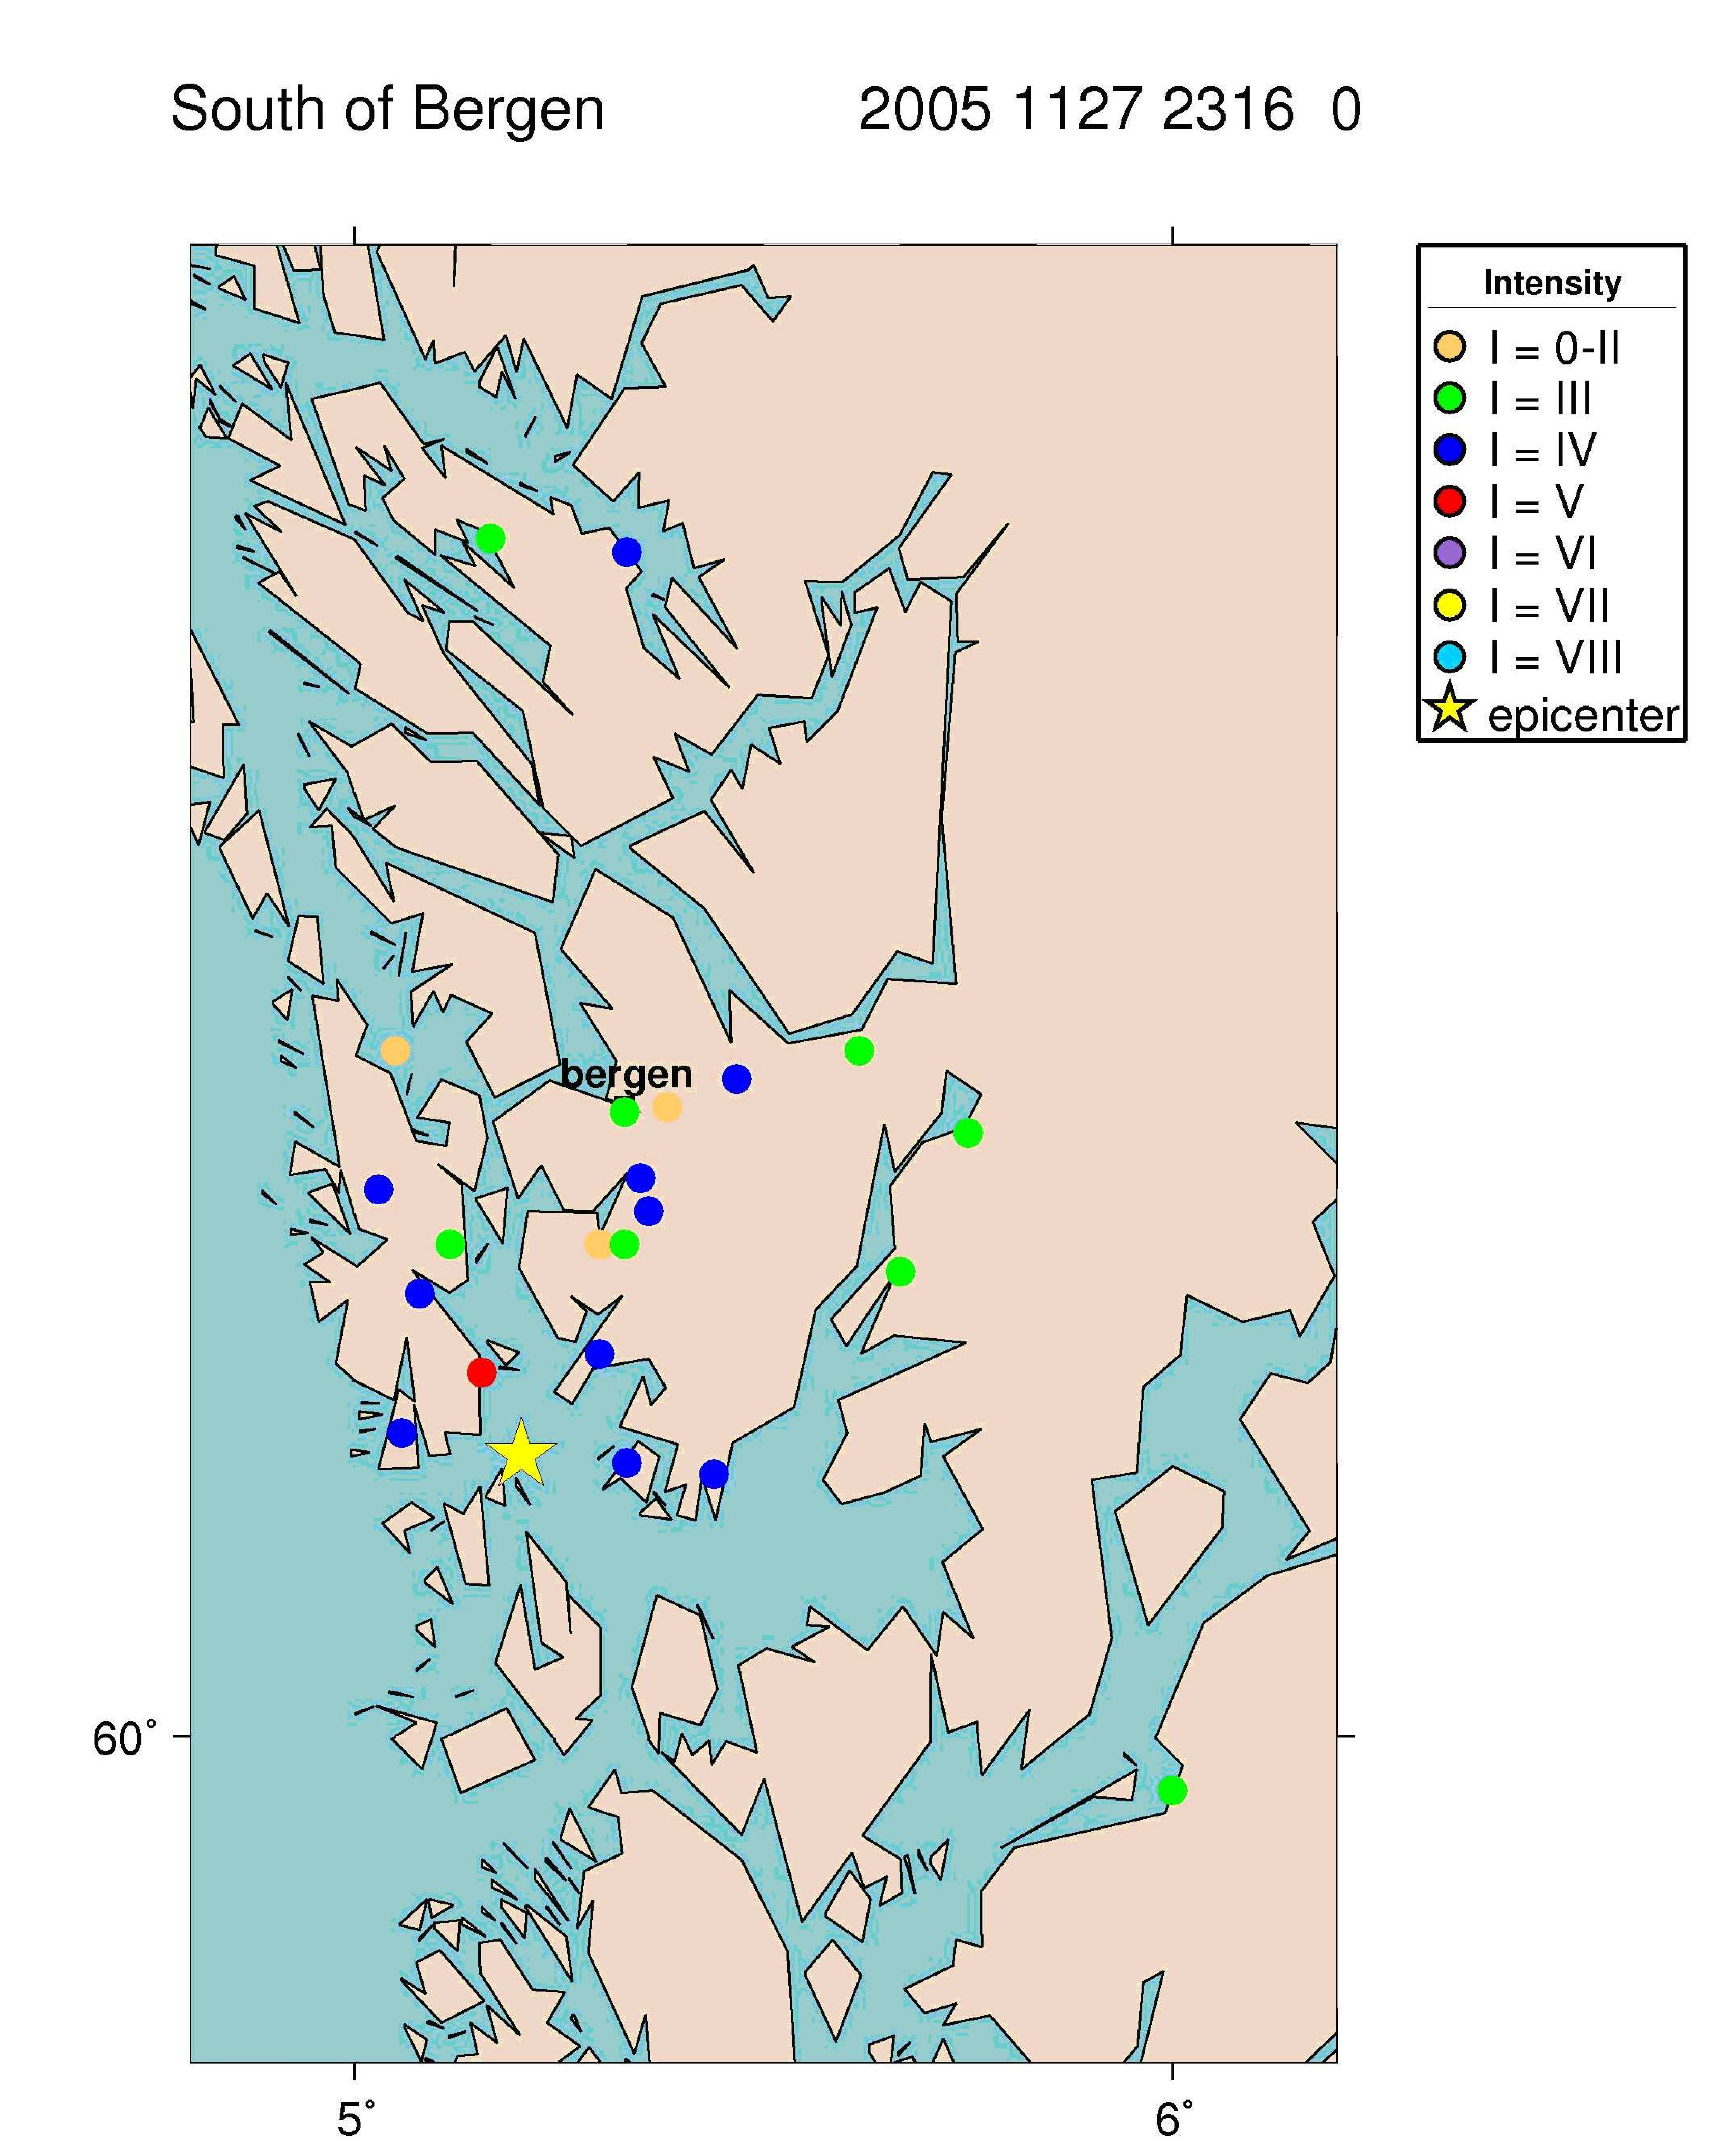
\includegraphics[width=0.9\linewidth]{fig/fig52}}
\caption{Macroseismic map made with MACROMAP using EEV. 
The epicenter, taken from the S-file, is shown with the star.}
%\label{fig:}
\end{figure}

An example of the postal code file is 

\verbatiminput{include/macro.fil}

The content is postal code, latitude, longitude and location. The format is a10,ff10.3,2x,a30. the postal code does not have to be a number, but can be any string. 

